%Geometry
% Easter Term 1995-1996

% Lectured by Dr. N.I. Shepherd-Barron
% LaTeXed (unofficially) by Paul Metcalfe

% Comments and corrections to soc-archim-notes@lists.cam.ac.uk

\documentclass{notes}

\theoremstyle{plain}
\newtheorem{proposition}{Proposition}[chapter]
\newtheorem{theorem}[proposition]{Theorem}
\newtheorem{corollary}[proposition]{Corollary}
\newtheorem*{example}{Example}
\newtheorem{definition}[proposition]{Definition}
\newtheorem*{examples}{Examples}
\newtheorem{lemma}[proposition]{Lemma}
\newtheorem*{notes}{N.B}
\newtheorem*{notation}{Notation}
\newtheorem*{remark}{Remark}

\DeclareMathOperator{\Stab}{Stab}
\DeclareMathOperator{\Orb}{Orb}
\DeclareMathOperator{\dist}{dist}
\DeclareMathOperator{\Area}{Area}

\newcommand{\Cinf}{\C_\infty}
\newcommand{\T}{\mathbb{T}}
\newcommand{\cM}{\mathcal{M}}
\newcommand{\cC}{\mathcal{C}}
\newcommand{\cP}{\mathcal{P}}

\begin{document}
\frontmatter
\title{Geometry}

\lecturer{Dr.~N.I.~Shepherd-Barron}
\maintainer{Paul Metcalfe}
\date{Easter 1996}

\maketitle

\thispagestyle{empty}
\noindent\verb$Revision: 1.3 $\hfill\\
\noindent\verb$Date: 1999/09/17 17:41:57 $\hfill\
\vspace{1.5in}

The following people have maintained these notes.

\begin{center}
\begin{tabular}{ r  l}
-- date & Paul Metcalfe
\end{tabular}
\end{center}

\tableofcontents

\chapter{Introduction}

These notes are based on the course ``Geometry'' given by
Dr.~N.I.~Shepherd-Barron in Cambridge in the Easter Term 1996.  These
typeset notes are totally unconnected with Dr.~Shepherd-Barron.

These notes are incomplete.  If you have a problem with this, then you
can sort them out yourself.  Dr.~Shepherd-Barron has an updated
version on his web page.

\alsoavailable
\archimcopyright

\mainmatter

\chapter{Spherical Trigonometry}

\section{Introduction}

Fix a sphere $S$ in $\R^3$ with centre $0$ and radius $1$.  A line on $S$ is
a great circle (e.g. the equator).  Given any two non-antipodal points $P$
and $Q$ on $S$, there exists just one great circle through $P$ and $Q$.  A
spherical triangle looks like

\begin{center}
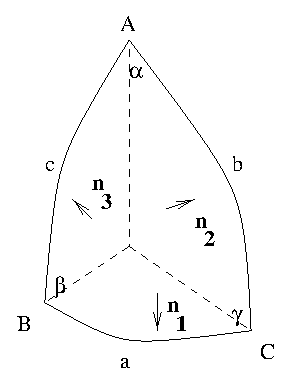
\includegraphics{sphtri.eps}
\end{center}

where $AB$, $BC$ and $AC$ are segments of great circles.  The length of the
line $AB$ is the angle subtended at $0$.  Any great circle is $S \cap H$, where
$H$ is a plane through the origin. $\alpha$ is defined as the angle between
the two relevant planes.

$\n_1$, $\n_2$ and $\n_3$ are the unit normals and
$\vect{A}$, $\vect{B}$ and $\vect{C}$ are the position vectors of $A$, $B$
and $C$.  Note that 
\begin{align*}
\n_1 = \frac{\vect{C} \times \vect{B}}{\sin a}
& &
\n_2 = \frac{\vect{A} \times \vect{C}}{\sin b}
& &\text{and} \quad
\n_3 = \frac{\vect{B} \times \vect{A}}{\sin c}.
\end{align*}

\begin{theorem}
$\sin a \sin b \cos \gamma = \cos c - \cos a \cos b$.
\end{theorem}

\begin{proof}
Use $(\vect{C} \times \vect{B}) \cdot (\vect{A} \times \vect{C})
= (\vect{A}\cdot\vect{C})(\vect{B} \cdot \vect{C})- (\vect{C}\cdot\vect{C})
(\vect{B}\cdot\vect{A})$.  Now $\abs{\vect{C}} = 1$, so
$(\vect{C} \times \vect{B})\cdot(\vect{A} \times \vect{C}) =
(\vect{A}\cdot\vect{C})(\vect{B}\cdot\vect{C})- (\vect{B}\cdot\vect{A})$.

Now
\begin{align*}
-\cos \gamma = \n_1 \cdot \n_2 &=
\frac{(\vect{C} \times \vect{B})\cdot(\vect{A} \times \vect{C})}{\sin a \sin b} \\
& = \frac{(\vect{A} \cdot\vect{C})
(\vect{B}.\vect{C})- (\vect{B} \cdot \vect{A})}{\sin a \sin b} \\
& = \frac{\cos b \cos a - \cos c}{\sin a \sin b}.
\end{align*}
\end{proof}

\begin{theorem}
$\sin \alpha \sin \beta \cos c = \cos \gamma + \cos \alpha \cos \beta$. 
\end{theorem}

\begin{proof}
Use the same identity on $\n_2 \times \n_3 = \vect{A} \sin \alpha$,
$\n_3 \times \n_1 = \vect{B} \sin \beta$ and
$\n_1 \times \n_2 = \vect{C} \sin \gamma$.  Now
\begin{align*}
\sin \alpha \sin \beta \cos c &=
(\n_2 \times \n_3) \cdot (\n_3 \times \n_1) \\
&= (\n_1 \cdot \n_3)(\n_2 \cdot \n_3) - (\n_1 \cdot \n_2)\\
&= \cos(\pi - \beta)\cos(\pi - \alpha) - \cos(\pi - \gamma) \\
&= \cos \gamma + \cos \alpha \cos \beta.
\end{align*}

\end{proof}

\begin{theorem}
\[
\frac{\sin a}{\sin \alpha} = \frac{\sin b}{\sin \beta} = 
\frac{\sin c}{\sin \gamma}.
\]
\end{theorem}

\begin{proof}
Use $(\vect{A} \times \vect{C}) \times (\vect{C} \times \vect{B})
= (\vect{C} \cdot (\vect{B} \times \vect{A})) \vect{C}$.

\begin{align*}
(\vect{A} \times \vect{C}) \times (\vect{C} \times \vect{B})
&= -(\n_1 \times \n_2) \sin a \sin b \quad \text{ and } \\
\n_1 \times \n_2 & = \vect{C} \sin \gamma \quad \text{ so } \\
- \sin a \sin b \sin \alpha\ \vect{C} &= (\vect{C} \cdot (\vect{B} \times \vect{A}))
\vect{C}.
\end{align*}

Now

\begin{align*}
\vect{C}\cdot(\vect{A} \times \vect{B}) & = \sin a \sin b \sin \gamma \\
\vect{A}\cdot(\vect{B} \times \vect{C}) & = \sin b \sin c \sin \alpha \\
\vect{B}\cdot(\vect{C} \times \vect{A}) & = \sin c \sin a \sin \beta.
\end{align*}

Divide by $\sin a \sin b \sin c$ to get result.
\end{proof}

These results can be compared to the Euclidean case, when $a$, $b$ and $c$ are
very small.  Theorem 1.1 gives the cosine rule, theorem 1.2 is uninteresting
and theorem 1.3 gives the sine rule.

The triangle inequality ($c \le a + b$) can also be deduced if $\alpha$,
$\beta$ and $\gamma$ are less than $\frac{\pi}{2}$ and $a$, $b$ and $c$ are
less than $\pi$.

\begin{align*}
\cos c - \cos a \cos b &= \sin a \sin b \cos \gamma \quad \text{so} \\
\cos c & \ge \cos a \cos b \\
& \ge \cos (a+b) \quad \text{thus} \\
c & \le a + b.
\end{align*}

\section{Areas of Spherical Triangles}

\begin{theorem}
Suppose $\Delta$ is a spherical triangle with angles $\alpha$, $\beta$ and
$\gamma$.  Then the area of $\Delta$ is $\alpha + \beta + \gamma - \pi$.
\end{theorem}

\begin{proof}
Suppose $A$ and $B$ are antipodal points on the unit sphere $S$ and suppose
we have two great circles through $A$ and $B$. These 2 circles cut $S$ into
4 pieces called lunes.

\begin{center}
\includegraphics{lune.eps}
\end{center}

The area of the lune is $4 \pi \frac{\alpha}{2 \pi} = 2 \alpha$.

\begin{center}
\includegraphics{triarea.eps}
\end{center}

$P'$, $Q'$ and $R'$ are the antipodes of $P$, $Q$ and $R$ respectively and
$\Delta_1'$, $\Delta_2'$ and $\Delta_3'$ are the antipodal triangles of
$\Delta_1$, $\Delta_2$ and $\Delta_3$ respectively.  $\Delta'$ is the antipodal
triangle of $\Delta$, which is the exterior of the figure shown.  Note
that $\Delta + \Delta_1$, $\Delta + \Delta_2$ and $\Delta + \Delta_3$ are lunes
with areas of $2 \alpha$, $2 \beta$ and $2 \gamma$ respectively\footnote{In an
abuse of notation $\Delta_X$ will be either the triangle or its area.}.

Now $S \subset \R^3$, and the transformation sending $x$ to its antipodes $x'$
is the matrix $-I$, which is area-preserving.  Thus $\Delta = \Delta'$ and so
on.  Hence $\Delta + \Delta_1 + \Delta_2 + \Delta_3 = \Delta' + \Delta_1' +
\Delta_2' + \Delta_3'$.  But these 8 triangles make up the whole sphere, and
thus $\Delta + \Delta_1 + \Delta_2 + \Delta_3 = 2 \pi$.  From the lunes,
$3 \Delta + \Delta_1 + \Delta_2 + \Delta_3 = 2 (\alpha + \beta + \gamma)$, and
thus $\Delta = \alpha + \beta + \gamma - \pi$.
\end{proof}

The area thus depends only on the angles.  But the sides determine the angles,
and thus the area.

\begin{theorem}[Polygons on the sphere]
Suppose $\Pi$ is an $n$-gon on $S$ with interior angles $\sigma_1, \dots,
\sigma_n$.  Then the area of $\Pi$ is $\sum_i \sigma_i - (n-2) \pi$.
\end{theorem}

\begin{proof}
Cut $\Pi$ into $n-2$ triangles (prove this is possible by induction).  Suppose
the angles of $\Delta_i$ are $\alpha_i$, $\beta_i$ and $\gamma_i$.  Then the
area of $\Pi$ is
\begin{align*}
\sum_{i=1}^{n-2} \Delta_i &= \sum_{i=1}^{n-2} (\alpha_i + \beta_i + \gamma_i)
-(n-2) \pi \\
&=\sum_{i=1}^n \sigma_n - (n-2) \pi. 
\end{align*}
\end{proof}

\begin{corollary}[Gauss-Bonnet Formula]
  Suppose that $S$ is cut into polygons labelled $\Pi_1, \dots,
  \Pi_F$.  Say there are $E$ edges and $V$ vertices in total.  Then $V
  - E + F = 2$.
\end{corollary}

\begin{proof}
Suppose that $\Pi_i$ has $n_i$ edges and its interior angles sum to $\tau_i$.
Note that $\sum \tau_i = 2 \pi V$ and $\sum_{i=1}^F n_i = 2 E$.  Then
\begin{align*}
4 \pi = \sum_{i=1}^F \Pi_i &= \sum_{i=1}^F (\tau_i - (n_i - 2) \pi) \\
& = 2 \pi ( V - E + F ).
\end{align*}

\end{proof}

\section{Sterographic projection of $S$ into $\C$}

Let $\Cinf = \C \cup \{ \infty \}$.  $\C$ has a co-ordinate $\zeta$.  Near the
point at infinity, use the co-ordinate $\omega = 1/\zeta$.  Thus to make
calculations at or near infinity, use $\omega$ instead of $\zeta$.

Consider $P \in S$ and $\phi : S \mapsto \Cinf$ be the map defined by
making $N$, $P$ and $\phi(P)$ colinear.  To get an explicit formula for $\phi$,
take $P = (x,y,z)$.  We know that $\phi(P) = t(x,y,z) + (1-t)(0,0,1)$ for some
$t \in [0,1]$.  Thus $zt + 1 - t = 0$ and $t = 1/(1-z)$ and

\[
\phi(P) = \left(\frac{x}{1-z}, \frac{y}{1-z}, 0 \right).
\]

\begin{notes}
$\zeta = \frac{x + \imath y}{1-z}$ and the north pole corresponds
to the point at infinity.
\end{notes}

Recall that $\Cinf$ has the group of M\"{o}bius transforms acting on it and
$S$ has $SO(3)$.  If $\left( \begin{matrix}
\alpha & \beta \\
\gamma & \delta \end{matrix} \right)$ is a $2 \times 2$ complex matrix with
non-zero determinant, then it acts on $\Cinf$ by
\[
\left( \begin{matrix}
\alpha & \beta \\
\gamma & \delta \end{matrix} \right) \zeta = 
\frac{\alpha \zeta + \beta}{\gamma \zeta + \delta}.
\]


\begin{theorem}
Via $\phi$, every rotation of $S$ gives rise to a M\"{o}bius transform on
$\Cinf$. (Not every M\"{o}bius transform comes from a rotation.)
\end{theorem}

\begin{proof}

Step 1.  Deal with rotations about the $z$ axis through an arbitrary angle
$\theta$ ($R_{z,\theta}$).  This is the same as rotating the complex plane
through $\theta$ about $0$, accomplished by
\[
\left(
\begin{matrix}
e^{\imath \theta/2} & 0 \\
0 & e^{- \imath \theta/2}
\end{matrix}
\right).
\]

Step 2.  Now look at a rotation $R_{y,-\frac{\pi}{2}}$.  This is a $3 \times 3$
orthogonal matrix
\[
\left(
\begin{matrix}
0 & 0 & 1 \\
0 & 1 & 0 \\
-1 & 0 & 0
\end{matrix}
\right),
\]
and $\zeta \mapsto \zeta' = \frac{z + \imath y}{1-x}$.  The M\"{o}bius
transform $\zeta \mapsto \frac{\zeta - 1}{\zeta + 1}$ does the trick.  (Proof
by churn.)

Step 3.  Now $R_{\nu, - \pi/2}$ for any horizontal $\nu$.  Set $\psi$ to be
the angle between $\nu$ and the y axis.  Then
\[
R_{\nu, - \pi/2} = R_{z, \phi} R_{y,- \pi/2} \left( R_{z ,\psi}
\right)^{-1},
\] and thus $R_{\nu, - \pi/2}$ gives a M\"{o}bius map.

Step 4.  Now a general rotation $R_{\nu, \theta}$.  Rotate $\nu$ about the
x axis to $\nu'$, which is horizontal.  Then $\nu' = R_{x,\psi} (\nu)$ for
some $\psi$.  Hence
\[
R_{\nu, \theta} = R_{x, \psi} R_{\nu',\theta} \left( R_{x,\psi} \right)^{-1},
\]
so the general rotation gives rise to a M\"{o}bius map.
\end{proof}

The question remains as to which M\"{o}bius transforms arise from rotations.
Rotations have 3 real degrees of freedom, whereas M\"{o}bius transforms have 6
($0$, $1$ and $\infty$ can each go anywhere on $\Cinf$).  In fact, M\"{o}bius
transforms arising from rotations are the ones given by $A \in SU(2)$.  A proof
is via quaternions.

\chapter{Reflexions and Tessellations}

Suppose that in Euclidean space $\R^n$ we have hyperplanes $H_1, \dots, H_N$
(not necessarily containing the origin), with unit normals $n_i$.  Each
$H_i$ divides $\R^n$ into two pieces; say $\R^n \setminus H_i = A_i^+ \cup
A_i^-$, with $A_i^+$ being ``the vectors on the same side as $n_i$''.  Put
$\cC = \cap_i A_i^+$.

Define the angle $\theta_{ij} \in [0,\pi)$ between $H_i$ and $H_j$ by
$n_i.n_j = - \cos \theta_{ij}$.  Let $s_i$ denote reflexion in $H_i$ and put
$S = \{ s_1, \dots, s_N\}$.  We shall be interested in the group
$W = W_S = \langle s_1, \dots, s_N \rangle$ generated by $S$ and how the
regions $w(\cC)$, where $w \in W$, fit together.

\begin{lemma}
If $H$ is a side of $\cC$ and $w \in W$, then ``reflexion in w(H)'' is an
element of $W$.
\end{lemma}

\begin{proof}
If $\sigma$ is reflexion in $H$, then $w \sigma w^{-1}$ is reflexion in
$w(H)$. 
\end{proof}

\begin{notation}
If $\sigma = s_i$, then we sometimes write $A_\sigma^\pm$, $H_\sigma$ instead
of $A_i^\pm$ and $H_\sigma$.
\end{notation}

\begin{notes}
$\sigma(A_\sigma^\pm) = A_\sigma^\mp$.
\end{notes}

\begin{definition}
For $w \in W$, define the \emph{S-length} of $w$, $\ell_s(w)$ as the least
$p \ge 0$ such that $w = s_{i_1}, \dots, s_{i_p}$, $s_{i_j} \in S$.
\end{definition}

\begin{notes}
If $T \subset S$ and $u \in W_T$, then $\ell_S(u) \le \ell_T(u)$.
\end{notes}

Assume now that every dihedral angle $\theta_{ij}$ is either a fraction of
$\pi$, $\theta_{ij} = \pi/m_{ij}$ for some $m_{ij} \in \N$ or $\theta_{ij}=0$.
In this latter case, we write $m_{ij} = \infty$.

\begin{lemma}
Suppose $s$, $s' \in S$, $s \neq s'$, $T = \{s,s'\}$ and $v \in W_T$.  Put
$A_s^+ \cap A_{s'}^+ = \cP$.  Then $v(P)$ is contained in either $A_s^+$ or
$A_s^-$ and in the latter case $\ell_T(sv) = \ell_T(v) - 1$. 
\end{lemma}

\begin{proof}
Suppose that $H$ and $H'$ are the hyperplanes corresponding to $s$ and $s'$
respectively.  There are 2 cases to consider.

Case 1: $H$, $H'$ are parallel.  Label the images $v(\cP)$ by the element $v$.
Clearly $v(\cP)$ lies in just one of the regions $A_s^+$, $A_s^-$.  Also,
$v(\cP) \subset A_s^-$ iff
\[
v \in \{s, s s', s s' s, s s' s s', \dots \}
\]
and in this case $\ell_T(sv) = \ell_T(v) - 1$.

Case 2.  The dihedral angle between $H$ and $H'$ is $\pi/m$, $m \in \N$.  Then
take a 2-plane $L$ perpendicular to $H \cap H'$ and divide $L$ into $2m$ equal
sectors by lines through $L \cap H \cap H'$, which we will regard as the origin
in $L$.  One of these sectors corresponds to $\cP$.

$W_T = \{1, s', s's, s'ss', \dots, u=(s's \dots) \} \cup \{ s, ss', ss's,
 \dots, w=(ss'\dots)\}$, where $\ell_T(u) = m-1$ and $\ell_T(w) = m$.  Note
that $W_T$ is $D_{2m}$, the dihedral group with $2 m$ elements or the symmetry
group of a regular $m$-gon.

$v(\cP)$ is clearly one of these sectors (draw a picture to convince
yourself), and so lies in just one of $A_s^+$, $A_s^-$.  Moreover,
$v(\cP) \subset A_s^-$ iff $v \in \{s, ss', \dots, w\}$, and thus
$\ell_T(s v) = \ell_T(v) - 1$.
\end{proof}

This next result is the main step in constructing tessellations of Euclidean
space and spheres.  By definition, a tessellation of a space is a partition of
it into disjoint congruent regions.  Sometimes it is demanded that these
regions have finite volume.

\begin{theorem}
If $w \in W$ and $w(\cC) \cap \cC$ is nonempty, then $w = 1$.
\end{theorem}

\begin{proof}
Non-examinable.
\end{proof}

\section{Regular Polyhedra}

We are now back in $\R^3$.  Assume $0 \in H_i\ \forall\ i$.  Take the unit
sphere $S$.  Each $H_i$ cuts $S$ in a great circle, and $\cC \cap S$ is a
spherical polygon $\Pi$.

If $N=3$ then $\Pi$ is a triangle, with angles $\alpha$, $\beta$, $\gamma =
\pi/p$, $\pi/q$, $\pi/r$ with $p$, $q$, $r \ge 2$.  The area of $\Pi$ is
$\pi \left( \frac{1}{p} + \frac{1}{q} + \frac{1}{r} - 1 \right)$, and so
$\frac{1}{p} + \frac{1}{q} + \frac{1}{r} > 1$.  Solve these equations to
get \begin{align*}
(p,q,r) = &(2,2,n), n \ge 2, \\
&(2,3,3) \\ &(2,3,4) \\ &(2,3,5).
\end{align*}

Identify reflection of $\R^3$ in $H$ with reflection of $S$ in $S \cap H$.
Let $W$ be the group generated by reflections in the sides of $\Pi$.  Claim
that $w(\Pi)$ will cover the sphere.  Suppose otherwise,  then somewhere on $S$
there is something like:
\begin{center}
\includegraphics{sphcov.eps}
\end{center}
Now reflect in $l$.  Thus we have covered the sphere with disjoint congruent
spherical triangles.

Take $(p,q,r) = (2,3,5)$.  Then the area of $\Pi$ is $\pi/30$.  Now $w(\Pi)$
tessellates $S$ with $\frac{4 \pi}{\pi/30} = 120$ triangles.  Use these
triangles to construct a regular icosahedron - that is a tessellation of $S$
by 20 congruent equilateral triangles.  Group together the 120 triangles 6 at
at time as shown:

\begin{center}
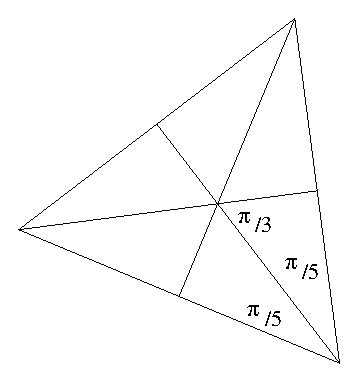
\includegraphics{icosa.eps}
\end{center}

How many vertices does the icosahedron have?  Now $V-E+F=2$, $E=30$, $F=20$,
so $V=12$.  So the sphere $S$ is tessellated into 20 congruent equilateral
triangles with angles $2 \pi / 5$.  There are 12 vertices and $5$ triangles
around each vertex.   $W$ is a group of symmetries of the icosahedron because
$W$ preserves the tessellation.  The 6-grouping is unique because the vertices
of the big triangles are those points surrounded by 10 little triangles.  So 
$W$ preserves the tessellation into 20 big triangles.

Also, $W$ acts transitively on faces, edges and vertices.

\begin{proof}[Proof for faces]
The elements of $W$ correspond to 120 small triangles, so $w \in W$ corresponds
to $w(\Pi)$. Now $\abs{W} = 120$, so $\abs{\Orb F} = \frac{120}{\Stab F}$ and
thus $\abs{\Orb F} \ge 20$, so $\abs{\Orb F} = 20$.  There is just one orbit,
so $W$ acts transitively on the faces.  The proof for edges and vertices is
similar.
\end{proof}

Also, given a vertex $P$, there are 5 faces around $P$.  $\Stab P$ acts
transitively on these 5 faces.  $\Stab P \cong D_{2 \times 5}$.

At the same time, we can construct a regular dodecahedron.  Take 10 small
triangles around $P$.  They form a regular pentagon, and by repeating we get
a tessellation of the sphere into 12 regular pentagons -- a regular dodecahedron
with symmetry properties analogous to those of the icosahedron.

\begin{center}
\begin{tabular}{c | c | c}
$(p,q,r)$ & shapes & number of little triangles \\
\hline
$(2,3,4)$ & cube and octahedron & 48 \\
$(2,3,3)$ & tetrahedron & 24 \\
$(2,2,n)$ &  & $4 n$
\end{tabular}
\end{center}

\chapter{Hyperbolic Geometry}

This is the third kind of 2D geometry where the group of isometries has 2
degrees of freedom.

\section{Riemannian Metrics}

Suppose $U \subseteq \R^2$ with co-ordinates $x$ and $y$.  Then a Riemannian
metric on $U$ is an expression $\ud s^2 = A\, \ud x^2 + 2 B\, \ud x\,
\ud y + C\, \ud y^2$ such that the matrix
\[
\left( \begin{matrix}
A & B \\
B & C
\end{matrix}
\right)\text{ is positive definite and } A > 0.
\]

Note that $A$, $B$ and $C$ are not necessarily constant.

Now $\ud s^2$ can be used to compute lengths of curves, angles between
curves and areas as follows.

Suppose $\Gamma$ is a path from $P$ to $Q$ in $U$, $\gamma : [0,1] \mapsto U$
with $\gamma(0) = P$ and $\gamma(1) = Q$.  Then the length of $\Gamma$ is
\begin{align*}
  \int_\gamma \ud s &= \int_{t=0}^1 \frac{\ud s}{\ud t} \ud t \\
  &= \int_{t=0}^1 \sqrt{A \left(\frac{\ud x}{\ud t}\right)^2 + 2 B\,
    \frac{\ud x}{\ud t}\frac{\ud y}{\ud t} + C \left(\frac{\ud y}{\ud
        t}\right)^2}\ \ud t,\text{ where } \gamma(t) = (x(t),y(t)).
\end{align*}

It is easy to show that if $\gamma'$ is a different parametrisation of
$\Gamma$, the length is found to be the same.

Now, suppose that $v = (v_1,v_2)$ and $w = (w_1, w_2)$ starting at $P$.  Then
define the angle $\theta$ between them by $v.w = \norm{v} \norm{w} \cos
\theta$, where $v.w$ =
\[
\left(
\begin{matrix}
v_1 & v_2
\end{matrix}
\right) \left(
\begin{matrix}
A(P) & B(P) \\
B(P) & C(P)
\end{matrix}
\right) \left(
\begin{matrix}
w_1 \\
w_2
\end{matrix}
\right).
\]

Define $\norm{v} = \sqrt{v.v}$.

If $\Gamma_1$ and $\Gamma_2$ are two curves meeting at $P$, then the angle
between them is defined to be the angle between their tangent vectors.

As for areas:  Suppose we have a small parallelogram in $U$.  Measure the
lengths and angles according to $\ud s^2$.  Then the area is $\sqrt{A C - B^2}\
\delta x\, \delta y$.  So given some subset $\Omega \subset U$, the area of
$\Omega$ is 
\[
\int_\Omega \sqrt{A C - B^2}\ \ud x\, \ud y.
\]

\begin{definition}
  Suppose $\ud s^2$ and $\ud u^2$ are 2 Riemannian metrics on $U$.
  They are said to be \emph{conformal} if $\ud s^2 = \phi \ud u^2$,
  where $\phi$ is differentiable and greater than $0$ on $U$.
\end{definition}

\begin{lemma}
  If $\ud s^2$ and $\ud\sigma^2$ are conformal then they define the
  same notion of angle.
\end{lemma}

\begin{proof}
  Let $\ud s^2 = A\, \ud x^2 + 2 B\, \ud x\, \ud y + C\, \ud y^2$ and
  $\ud\sigma^2 = \alpha\, \ud x^2 + 2 \beta\, \ud x\, \ud y + \gamma\,
  \ud y^2$.

Let $v = \left(\begin{matrix}v_1 \\ v_2 \end{matrix} \right)$ and
$w = \left(\begin{matrix}w_1 \\ w_2 \end{matrix} \right)$.

Call the angle between $v$ and $w$ defined by $\ud s^2$ $\theta_1$ and
the angle between $v$ and $w$ defined by $\ud\sigma^2$ $\theta_2$.
Similarly, let $\norm{v}_1$ be the norm defined by $\ud s^2$ and
$(v.w)_1$ be the dot product from $\ud s^2$ (and so on for
$\norm{v}_2$ and $(v.w)_2$).

Now
\begin{align*}
(v.w)_1 &= \norm{v}_1 \norm{w}_1 \cos \theta_1 \\
&= v^T \left( \begin{matrix}A & B \\ B & C \end{matrix} \right) w \\
&= \phi v^T \left( \begin{matrix}\alpha & \beta \\ \beta & \gamma \end{matrix}
\right) w \\
&= \phi (v.w)_2 \\
\Rightarrow \phi(P) (v.w)_2 &= \phi(P) \norm{v}_2 \norm{w}_2 \cos \theta_1 \\
&=\norm{v}_2 \norm{w}_2 \cos \theta_2 \\
\Rightarrow \cos \theta_2 &= \cos \theta_1
\end{align*}
\end{proof}

\section{The Hyperbolic Plane}

\begin{definition}
Define the hyperbolic plane $H$ as $\{ z \in \C \mid \Im z > 0 \}$.
\end{definition}

\begin{definition}
Define $\ud s^2 = \frac{\ud x^2 + \ud y^2}{y^2}$ -- the hyperbolic metric.
\end{definition}

The notion of angle is the same as in the Euclidean case, but lengths and
areas are different.

An isometry of $H$ is one which preserves the hyperbolic metric - that
is if $g(x,y) = (\xi, \eta)$, then $\frac{\ud x^2 + \ud y^2}{y^2} =
\frac{\ud\xi^2 + \ud\eta^2} {\eta^2}$.

Let
\[
G = \left\{
\left(
\begin{matrix}
\alpha & \beta \\ \gamma & \delta
\end{matrix}
\right) \mid \alpha, \beta, \gamma, \delta \in \R, \alpha \delta - \beta \gamma
= 1
\right\} = SL_2(\R).
\]

Now $G$ acts as a group of M\"{o}bius transforms on $\Cinf$ and preserves the
real line $\R$.  Thus $G$ acts as a group of M\"{o}bius transforms on $H$,
and preserves $\C \setminus \R = H \cup H_-$.  (Need to check that $g \in G$
cannot flip $H$ and $H_-$ -- not hard.)

\begin{proposition}
$G$ preserves the hyperbolic metric.
\end{proposition}

\begin{proof}
We will work with $z$ and $\Bar{z}$, thus
\[
\ud s^2 = \frac{\ud z\, \ud\Bar{z}}{\left( (z-\Bar{z})/2\imath \right)^2} =
\frac{-4\, \ud z\, \ud\Bar{z}}{(z-\Bar{z})^2}.
\]

Now take $g = \left(
\begin{matrix}
\alpha & \beta \\ \gamma & \delta
\end{matrix}
\right)$ and set
$\zeta = g(z) = \frac{\alpha z + \beta}{\gamma z + \delta}$.

Now
\[
\ud\zeta = \frac{\alpha\,\ud z\,(\gamma z + \delta) - \gamma\,\ud z\,(\alpha z +
\beta)}{(\gamma z + \delta)^2} = ( \gamma z + \delta)^{-2} \ud z,
\]
and $\ud\Bar{\zeta} = ( \gamma \Bar{z} + \delta)^{-2} \ud\Bar{z}$.  Then put
everything together -- it works!
\end{proof}

\begin{definition}
A hyperbolic line in $H$ (or a $H$-line) is either a semi-circle meeting $\R$
at right-angles or a vertical line.  We shall see that these $H$-lines minimize
distance in $H$.
\end{definition}

It follows from facts about circles that given two $H$-lines $L$ and $M$ there
are 3 possibilities.

\begin{enumerate}
\item $L$ meets $M$ at 1 point in $H$.
\item $L$ meets $M$ at 1 point in $\R \cup \{ \infty \}$.  In this case, $L$
and $M$ are said to be parallel.
\item $L$ and $M$ do not meet -- they are said to be ultraparallel.
\end{enumerate}

If $L$ and $M$ are not ultraparallel then we can define an angle between them.
In case 1, take it to be the Euclidean angle between them, otherwise the
angle is 0.

\begin{definition}
A hyperbolic triangle is a region defined by 3 $H$-lines, no two of which
are ultraparallel.
\end{definition}

\begin{example}\hfill
\begin{center}
\includegraphics{htri1.eps}
\end{center}
$\Delta$ has three angles, $\alpha$, $\beta$ and $\gamma$ -- $\gamma = 0$.
\end{example}

\begin{proposition}
The area of $\Delta$ is $\pi - (\alpha + \beta + \gamma)$.
\end{proposition}

To prove this, we need a few facts about maps preserving the Riemannian metric.
Suppose $\gamma$ is a curve from $P$ to $Q$, and $g$ takes $\gamma$ to
$\gamma_1$.  Now $g$ preserves $\ud s^2$, so $\ud s$ is preserved and so is
\[
\int \ud s = \text{length}.
\]

Now given $\Omega \subset U$, the area of $\Omega$ is
\[
\int_\Omega \sqrt{A C - B^2}\ \ud x\, \ud y.
\]

Let $g(x,y) = (\xi,\eta)$, so that
\[
\ud s^2=
\left(
\begin{matrix}
\ud\xi & \ud\eta
\end{matrix}
\right) \left(
\begin{matrix}
\alpha & \beta \\
\beta & \gamma
\end{matrix}
\right) \left(
\begin{matrix}
\ud\xi \\
\ud\eta
\end{matrix}
\right)
=
\left(
\begin{matrix}
\ud x & \ud y
\end{matrix}
\right) \left(
\begin{matrix}
A & B \\
B & C
\end{matrix}
\right) \left(
\begin{matrix}
\ud x \\
\ud y
\end{matrix}
\right).
\]

Now
\[
\left(
\begin{matrix}
\ud\xi \\ \ud\eta
\end{matrix}
\right)
=\left(
\begin{matrix}
\pd{\xi}{x} & \pd{\xi}{y} \\
\pd{\eta}{x} & \pd{\eta}{y}
\end{matrix}
\right)
\left(
\begin{matrix}
\ud x \\ \ud y
\end{matrix}
\right) = J \left(
\begin{matrix}
\ud x \\ \ud y
\end{matrix}
\right).
\]

So
\[
J^T \left(
\begin{matrix}
\alpha & \beta \\
\beta & \gamma
\end{matrix}
\right) J = \left(
\begin{matrix}
A & B \\
B & C
\end{matrix}
\right),
\]
and thus $(\det J)^2 (\alpha \gamma - \beta^2) = A C - B^2$ and
$\sqrt{A C - B^2} = \abs{\det J} \sqrt{\alpha \gamma - \beta^2}$.  So the
area of $\Omega$ is
\[
\int_\Omega \sqrt{A C - B^2}\ \ud x\, \ud y = \int_{g(\Omega)} \abs{\det J}
\sqrt{\alpha \gamma - \beta^2}\ \ud x\, \ud y =
\int_{g(\Omega)} \sqrt{\alpha \gamma - \beta^2}\ \ud\xi\, \ud\eta,
\]
which is the area of $g(\Omega)$.

We are now in a position to prove the proposition.

\begin{proof}
$\exists\ g \in G$ taking a side of $\Delta$ to a vertical line.  If
one of the sides of $\Delta$ is a semi-circle from $P=(t,0)$ to $Q$, then
$g = \left(
\begin{matrix}
1 & -t \\ 0 & 1
\end{matrix}
\right)$ shifts $P$ to $0$.  Thus we may assume that $P = 0$.  Now if $Q =
(s,0)$, $g = \left(
\begin{matrix}
-1 & 0 \\ s^{-1} & -1
\end{matrix}
\right)$ shifts $Q$ to $\infty$.

Now, we may assume we have something looking like:

\begin{center}
\includegraphics{htri2.eps}
\end{center}

\[
\Area(\Delta + \Delta_1) = \int_{\Gamma_1 + \Gamma_2 + \Gamma_3}
\frac{\ud x}{y}
= \int_{\Gamma_2} \frac{\ud x}{y}.
\]

\begin{center}
\includegraphics{htri3.eps}
\end{center}

Put $z = r e^{\imath \theta}$, so $\ud x = -r \sin \theta \ud\theta$ and 
$y = r \sin \theta$.  Thus the required integral is
\[
\int_{\Gamma_2} -\ud\theta = \int_{\pi - \phi}^\omega - \ud\theta
= \pi - (\phi + \omega).
\]

Thus the area of $\Delta_1$ is $\pi - (\pi - \beta + \delta)$ and the
area of $\Delta + \Delta_1$ is $\pi - (\alpha + \gamma + \delta)$.  Thus
the area of $\Delta$ is $\pi - (\alpha + \beta + \gamma)$.
\end{proof}

\section{Another look at the hyperbolic plane}

Now introduce $\Delta = \{ z \in \C \mid \abs{z} < 1 \}$ with
$\ud\sigma^2 = \frac{4\, \ud z\, \ud\Bar{z}}{(1-z\Bar{z})^2}$.  We
firstly want to find a M\"{o}bius map $\psi$ taking $\Delta$ to $H$
and we then want to show that $\psi$ is an isometry.

Now there exists a unique M\"{o}bius map with the properties that:
\begin{align*}
-1 &\mapsto 0, \\
0 &\mapsto \imath \text{ and} \\
1 &\mapsto \infty.
\end{align*}

Let $\psi(z)$ be this map, that is $\psi(z) = -\imath \frac{z+1}{z-1}$.  Now
$\psi(\imath)$ is real, so $\psi$ must take the unit circle to $\R \cup
\{ \infty \}$.  Thus $\psi$ must take $\Delta$ to either $H$ or $H^-$.  But
$\psi(0) = \imath$, so $\psi$ takes $\Delta$ to $H$.

A hyperbolic line in $\Delta$ is a circle meeting $\partial \Delta$ at
right-angles.  Since $\psi$ is M\"{o}bius, it takes hyperbolic lines in
$\Delta$ to hyperbolic lines in $H$.

\begin{proposition}
$\psi$ is an isometry.
\end{proposition}

\begin{proof}
Let $\psi(z) = \zeta$.  Then $\frac{\ud x^2 + \ud y^2}{y^2} = \frac{-4 \ud\zeta\,
\ud\Bar{\zeta}}{(\zeta-\Bar{\zeta})^2}$.  Then
\begin{gather*}
  \ud\zeta = \frac{-\imath\, \ud z (z-1) + \imath (z+1) \ud
    z}{(z-1)^2} = \frac{2 \imath
    \, \ud z}{(z-1)^2}\\
  \ud\Bar{\zeta} = \frac{-2 \imath\, \ud\Bar{z}}{(\Bar{z}-1)^2}.
\end{gather*}

Now, substituting for $\ud\zeta$ and $\ud\Bar{\zeta}$, we get
\[
\frac{\ud x^2 + \ud y^2}{y^2} = \frac{4\, \ud z\, \ud\Bar{z}}{(1-z\Bar{z})^2},
\]
and thus $\psi$ is an isometry.
\end{proof}

On $H$ we have $G = SL_2(\R)$ preserving $\ud s^2$.  Thus $\psi^{-1} g \psi$
is a M\"obius transform from $\Delta$ to $\Delta$ preserving $\ud\sigma^2$.  So
$\Gamma = \{ \psi^{-1} g \psi \mid g \in G \}$ acts as a group of M\"obius
transforms on $\Delta$ preserving $\ud\sigma^2$.  These are the $2 \times 2$
complex matrices $A$ such that
\[
A^* J A = J,\text{ where } J = \left( \begin{matrix}
1 & 0 \\ 0 & -1
\end{matrix}\right).
\]

\begin{notes}
In $\Gamma$, $\Stab 0 = \left\{ \left( \begin{matrix}
e^{\imath \theta/2} & 0 \\ 0 & e^{-\imath \theta/2}
\end{matrix}\right) \mid \theta \in \R \right\}$
\end{notes}

\begin{proposition}
In $\Delta$ and $H$, given $P \neq Q$, $\exists!$ hyperbolic line joining
$P$ to $Q$.
\end{proposition}

\begin{proof}
We will prove this in $\Delta$.

If $P=0$ the hyperbolic lines are precisely the diameters, so given $Q \neq 0\
\exists!$ diameter through $Q$. 

If $P = \zeta \neq 0$, claim $\exists\ \gamma \in \Gamma$ such that
$\gamma(\zeta) = 0$.  To show this, go back to the upper half plane.  We
must show that given $z \in \C, \exists\ g \in G$ such that $g(z) = \imath$.
Let $z = x + \imath y$, and then put
\[
g = \left( 
\begin{matrix}
\sqrt{y} & \frac{x}{\sqrt{y}} \\
0 & \frac{1}{\sqrt{y}}
\end{matrix}
\right)^{-1}.
\]
This works, and reduces the problem to the previous case.
\end{proof}

Now we want to define a distance in $\Delta$ or $H$.  If $P \neq Q$ we will
define the distance from $P$ to $Q$ as the length\footnote{Measured according
to $\ud s^2$ or $\ud\sigma^2$.} of the unique hyperbolic line joining $P$ and $Q$,
and $0$ if $P = Q$.  We will compute this in $\Delta$ when one point $P = 0$.
Put $Q$ on $\R^+$ (say $Q = X$).  Call the $H$-line joining $P$ and $Q$
$\gamma$.

\[
\ell(\gamma) = \int_P^Q \ud s.
\]

\[
\text{Also, }\ud s = \sqrt{\ud\sigma^2} = \frac{2 \sqrt{\ud\zeta\, \ud\Bar{\zeta}}}{1 -
\zeta\Bar{\zeta}} = \frac{2 \ud x}{(1-x^2)}.\quad \text{Thus}
\]

\[
\ell(\gamma) = 2 \int_{t=0}^X \frac{\ud t}{1-t^2} = \log \frac{1+X}{1-X}.
\]

\section{Geodesics}

We want to find the paths which minimise distance in $\Delta$.  We shall use
the calculus of variations to minimise
\[
\int \ud s = \int \frac{\ud s}{\ud t}\, \ud t.
\]

Now $\frac{\ud s}{\ud t} = \frac{2(\dot{x}^2 + \dot{y}^2)^{1/2}}{1-( x^2 + y^2)}$,
thus we wish to minimise

\[
\int \frac{2(\dot{x}^2 + \dot{y}^2)^{1/2}}{1-( x^2 + y^2)} \ud t.
\]

Use polars, so that $x = r \cos \theta$ and $y = r \sin \theta$, to get
\[
F = \frac{2 (\dot{r}^2 + r^2 \dot{\theta}^2)^{1/2}}{1-r^2}.
\]
Thus, by the Euler-Lagrange equations
\begin{gather*}
\frac{\ud}{\ud t} F_{\dot{r}} = F_r \\
\frac{\ud}{\ud t} F_{\dot{\theta}} = F_\theta.
\end{gather*}

By applying a M\"obius map we may assume that $P=0$.

Now $F_\theta = 0$, so $\frac{\ud}{\ud t} F_{\dot{\theta}} = 0$.  Now
$F_{\dot{\theta}} = \frac{(\dot{r}^2 + r^2 \dot{\theta}^2}{1-r^2}$, and
evaluating at $r = 0$ gives that $F_{\dot{\theta}} = 0$, so $\dot{\theta}=0$.

Thus in $\Delta$, the geodesics are the hyperbolic lines.  It is an obvious
corollary that the same result holds in $H$.

\begin{notes}
Given $P$, $Q \in \Delta$, the distance from $P$ to $Q$ gives a metric
(in metric space sense).
\end{notes}

\begin{theorem}
Take $P \in \Delta$ and fix $r > 0$.  Then the hyperbolic circle $C$
with hyperbolic centre $P$ and hyperbolic radius $r$ 
(that is $\{ z \in \Delta : d_{hyp}(P,z) = r \}$) is a Euclidean circle,
but possibly with a different centre and radius.
\end{theorem}

\begin{proof}
We may assume that $P = 0$ (otherwise apply a M\"obius isometry -- which
preserves both Euclidean and hyperbolic circles).

If $h$ is M\"obius and in $\Stab 0$ then $h(C) = C$.  But then $h$ is a
rotation, so $C$ is rotationally invariant and thus a Euclidean circle.
\end{proof}

\begin{theorem}
In $\Delta$, Euclidean circles are hyperbolic circles.
\end{theorem}

\begin{proof}
Given a Euclidean circle $C$ in $\Delta$, we may rotate it so that its centre
is on $\R$, so we may assume that its centre is on $\R$.  Now consider the
M\"obius isometries
\[
\left\{
\left(
\begin{matrix}
\cosh t & \sinh t \\
\sinh t & \cosh t
\end{matrix}
\right) \mid t \in \R
\right\}
\]

Consider $g_t(C)$.  For $t \gg 0$, the centre of $g_t(C) > 0$ and for
$t \ll 0$ the centre of $g_t(C) < 0$.  So $\exists\ t' \in \R$ such that
the centre of $g_{t'}(C)$ is $0$.

We may now assume that $C$ is centred about $0$.  $C$ is now rotationally
invariant about $0$ -- but these are M\"obius isometries, so that $C$ is a
hyperbolic circle.
\end{proof}

The obvious corollary is that in $H$, Euclidean circles are hyperbolic circles.

\begin{theorem}
Any invertible holomorphic map $g : \Delta \mapsto \Delta$ (or $H \mapsto H$)
is M\"obius.  Any isometry $\Delta \mapsto \Delta$ (or $H \mapsto H$) is either
holomorphic or has a holomorphic conjugate.
\end{theorem}

\begin{proof}[Idea of proof]
$g$ preserves $\ud s^2$ and thus geodesics.  So it takes $H$-lines to $H$-lines.
Then show that $g$ is determined by 3 points.  Then show that 2 triples can
be mapped to each other by a M\"obius transformation.
\end{proof}

\section{Hyperbolic Trigonometry}

We now show another model of the hyperbolic plane.  In $\R^3$ consider $\Omega$
defined by $x^2 + y^2 - z^2 = -1$ and $z > 0$.  Define a map $\psi$ from
$\Omega$ to $\Delta$,
\[
(x,y,z) \mapsto \frac{x + \imath y}{z + 1}.
\]

Then hyperbolic lines in the disc correspond to planes through $0$ which cut
$\Omega$.  We define a new dot product on $\R^3$,
\[
\left<
\left(
\begin{matrix} x \\ y \\ z \end{matrix}
\right),
\left(
\begin{matrix} a \\ b \\ c \end{matrix}
\right)
\right> = a x + b y - c z.
\]

Then \[
\Omega = \left\{
u = \left(
\begin{matrix} x \\ y \\ z \end{matrix}
\right) \in \R^3 \mid u.u = -1, z > 0
\right\}.
\]

There is a notion of cross product such that
\[
u.(v \times w) = \left|
\begin{matrix}
u_1 & v_1 & w_1 \\
u_2 & v_2 & w_2 \\
u_3 & v_3 & w_3
\end{matrix}
\right|,
\]
with the properties that $v \times w = - w \times v$ and
$(x \times y) . (z \times t) = (x.t) (y.z) - (x.z) (y.t)$.

Consider the group $\Gamma$ of linear maps which preserve the dot product
with determinant $+1$.  Then $A \in \Gamma$ iff $A^T J A = J$, where
\[
J = \left(
\begin{matrix}
1 & 0 & 0 \\
0 & 1 & 0 \\
0 & 0 & -1
\end{matrix}
\right),\text{ as before.}
\]

The positive determinant prevents $A$ from flipping $\Omega$ to its opposite
with $z < 0$.

\begin{proposition}
Elements of $\Gamma$ correspond by $\psi$ to M\"obius isometries of $\Delta$.
(That is, given $A \in \Gamma$, $\psi A \psi^{-1}$ is M\"obius.)
\end{proposition}

\begin{proof}
First we construct a Riemannian metric on $\Omega$ such that $\psi$ is an
isometry --- $\ud\sigma^2 = \ud x^2 + \ud y^2 - \ud z^2$ does the trick.  It is not
Riemannian on $\R^3$ (it's Lorentzian), but its restriction to $\Omega$ is
Riemannian.  On $\Omega$, $x\, \ud x + y\, \ud y - z\, \ud z = 0$, substitute
for $\ud z$ in $\ud\sigma^2$.

Let $\zeta = \psi(x,y,z) = \frac{x + \imath y}{z+1}$.  Now
\[
\ud\zeta = \frac{(z+1)\, \ud z - x\, \ud z + \imath (z+1)\, \ud y -
  y\, \ud z}{(z+1)^2},
\]
and on $\Delta$ $\ud s^2 = \frac{4\, \ud\zeta\, \ud\Bar{\zeta}}{(1-\zeta \Bar{\zeta})
^2}$.  Substitute away... it works!

Now, suppose $L$ is a plane in $\R^3$ with $0 \in L$ and $L \cap \Omega \neq
\emptyset$.  If $(0,0,1) \in L$, then $\psi(L \cap \Omega)$ is a straight line
$\lambda \xi + \mu \eta = 0$, with $\zeta = \xi + \imath \eta$.  For general
$L$, $\exists\ $ many $A \in \Gamma$ such that $(0,0,1) \in A(L)$. Now
$A(L) \mapsto$ a hyperbolic line, say $M$, so $L \mapsto \psi A^{-1}
\psi^{-1} (M)$, which is a hyperbolic line.
\end{proof}

We can use $\Omega$ to derive formulae in $\Delta$.

\begin{proposition}
If $\zeta, \zeta_1 \in \Delta$, with $\zeta = \psi(u)$ and $\zeta_1 =
\psi(u_1)$ then $\dist(\zeta,\zeta_1) = \cosh^{-1} - u.u_1$.
\end{proposition}

\begin{proof}
The LHS is invariant under M\"obius isometries and the RHS is invariant
under $\Gamma$.  Therefore we may assume that $\zeta_1 = 1$ so that
$u_1 = (0,0,1)$.  Then if $\zeta = \frac{x + \imath y}{z+1}$, $-u.u_1
= z$.  Now $\cosh \dist(0,\zeta) = z$, so we have proved that
\[
\dist(0,\zeta) = \log \abs{ \frac{1+\abs{\zeta}}{1-\abs{\zeta}} }.
\]
\end{proof}

\section{Hyperbolic Trigonometry}

In $\Omega$ we have:
\begin{center}
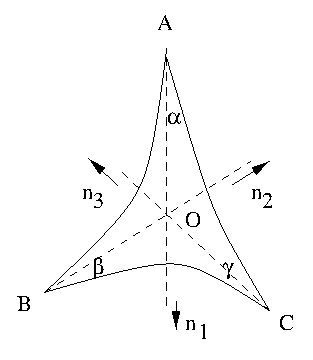
\includegraphics{htri4.eps}
\end{center}

$A$, $B$, $C \in \Omega$ and $\alpha$, $\beta$, $\gamma$ are the angles in the
image in $\Delta$.

We want to find these formulae, analogous to those found in the spherical case:

\begin{gather*}
\sin \alpha \sin \beta \cosh c = \cos \gamma + \cos \alpha \cos \beta \\
\sinh a \sinh b \cos \gamma = - \cosh c + \cosh a \cosh b \\
\frac{\sin a}{\sinh \alpha} = \frac{\sin b}{\sinh \beta} =
\frac{\sin c}{\sinh \gamma}
\end{gather*}

We can make $\n_i \cdot \n_i = 1$, since vectors pointing out of the
cone are positive.

\begin{lemma}
\[
\n_1 \times \n_2 = - \sin \gamma C
\]
\end{lemma}

\vspace{2in}

\begin{center}
\LARGE
Unfinished
\end{center}

If you've got this far... the book by Rees is probably the best for
this course.  When you've read and understood it, you can complete
these notes and remove all of the errors in the previous $N$ pages.

\begin{flushright}
\parbox{1in}{Have fun,\\Paul}
\end{flushright}

\end{document}
